\pagestyle{fancy}
\fancyhead[R]{Física Nuclear y de Partículas: Tema 5}
\fancyhead[L]{4º Grado en Física}
\chapter{Modelos del Núcleo}
Como ya hemos visto, los núcleos atómicos presentan una estrctura en sus energías de separación de manera muy parecida a cómo los átomos presentan sus energías de ionización, lo que nos sugiere que al igual que el modelo atómico tenía una estructura de capas, el núcleo también ha de tener una estructura similar.
\section{Estructura de capas. Números mágicos}
A la hora de entender un núcleo, no podemos obviar una serie de números en los cuales el núcleo presenta unas propiedades muy especiales, los \textbf{números mágicos} los cuales fueron presentados en el tema 3.
\\\\
El hecho de que existan los números mágicos nos dice que los nucleones se disponen en capas dentro del núcleo, así el modelo más efectivo para estudiar los núcleos atómicos es el \textbf{modelo de capas}\\\\
El modelo de capas se aplica sin modificaciones para los núcleos par-par, pues todos tienen $J^P=0^+$ en su estado fundamental; y con hipótesis adicionales (regla de Nordheim) para los núcleos impar-impar y para los núcleos con $A$ impar.\\\\
Este modelo es una teoría de campo medio (teoría efectiva), es decir, que cada nucleón se mueve en un potencial generado por el resto de nucleones; recordemos que la fuerza nuclear satura, por lo que el potencial que ven todos los nucleones (salvo superficie) es el mismo. Por lo tanto al construir dicho potencial, hemos de exigir que nos reproduzca de manera natural los números mágicos. Estos números son $$Z/N=2,8,20,28,50,82,126$$ y hablamos de núcleos \textbf{doblemente mágicos} cuando tanto sus protones y sus neutrones tienen un número mágico de ocupación \textit{e.g} oxígeno-16 $(8p,8n)$; mientras que hablamos de núcleos \textbf{simplemente mágicos} cuando sólo uno de los distintos nucleones tiene un número mágico de ocupación \textit{e.g} flúor-17 $(9p,8n)$.

\noindent
\begin{minipage}{0.55\textwidth}
\subsubsection{Evidencias empíricas del modelo de capas}
Si analizamos de esta manera la desviación de la masa respecto a la calculada con la fórmula semiempírica, vemos que las desviaciones más grandes se dan precisamente en los números mágicos.
\\\\
Existen muchas evidencias experimentales para suponer la estructura de capas.\\\\
En la figura \ref{fig: Seccion eficaz captura neutronica} vemos que cuando tenemos núcleos mágicos en neutrones, la sección eficaz es muy baja.\\\\
En la figura \ref{fig: Energias de separacion} vemos que las energías de separación se hacen máximas en los números mágicos.\\\\
En la figura \ref{fig: Energias de alfa vs neutrones} observamos una discontinuidad en $N=126$.
\\\\
En la figura \ref{fig: Radios de carga nuclear equivalente y numeros magicos} vemos que éstos se hacen pequeños al pasar por los números mágicos, que traducido al factor de forma, los núcleos atómicos se vuelven más esféricamente simétricos en las inmediaciones de los números mágicos.
\begin{center}
         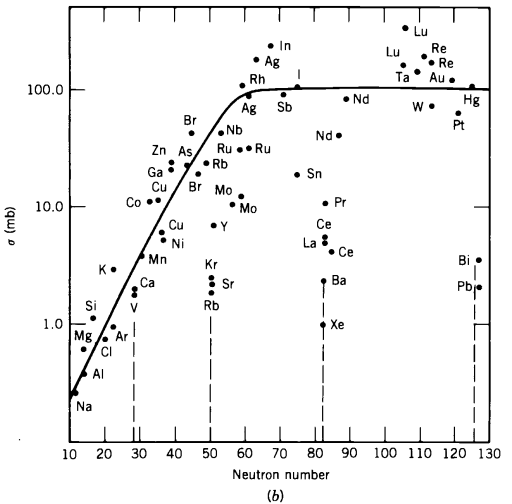
\includegraphics[width=\textwidth]{Diagramas Tema 5/Seccion eficaz vs neutrones.png}
        \captionof{figure}{Sección eficaz de captura neutrónica de varios núcleos.} 
    \label{fig: Seccion eficaz captura neutronica}
\end{center}
\end{minipage}
\hfill
\begin{minipage}{0.4\textwidth}
        \centering
    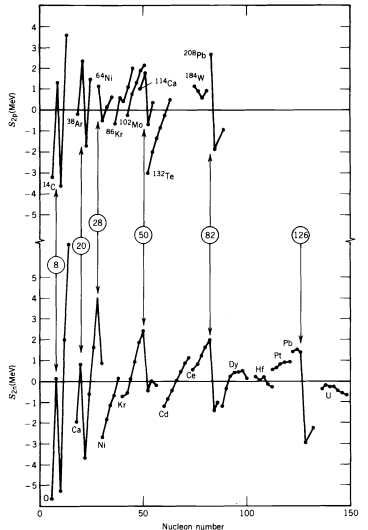
\includegraphics[width=\textwidth]{Diagramas Tema 5/Energias de separacion en funcion vs A.png}
    \captionof{figure}{(Arriba) Energías de separación de dos protones para secuencias de isótopos. Se indica el miembro de menor $Z$. (Abajo) Energías de separación de dos neutrones.}
    \label{fig: Energias de separacion}
\vfill
    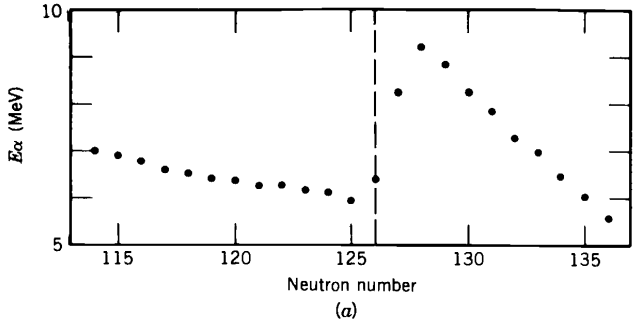
\includegraphics[width=\textwidth]{Diagramas Tema 5/Energia desintegracion alfa vs neutrones.png}
        \captionof{figure}{Energías de las partículas $\alpha$ emitidas por isótopos de Rn.} 
    \label{fig: Energias de alfa vs neutrones}
\vfill
    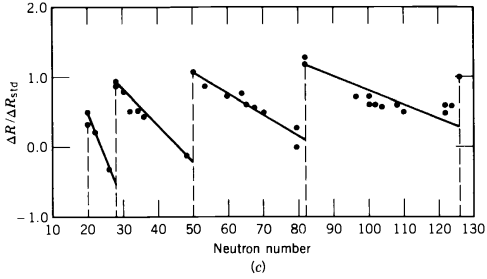
\includegraphics[width=\textwidth]{Diagramas Tema 5/Diferencias radio de carga equivalente.png}
        \captionof{figure}{Cambios en el radio de carga nuclear equivalente cuando tenemos $\Delta N=2$.} 
    \label{fig: Radios de carga nuclear equivalente y numeros magicos}
\end{minipage}
\newpage
\subsection{El potencial del modelo de capas}
A la hora de determinar el potencial que tiene el núcleo atómico, podemos pensar en distintos potenciales triviales para ver cómo reproducen los números de estados de ocupación
\subsubsection{Pozo esférico 3D}
\noindent
\begin{minipage}{0.6\textwidth}
El primer potencial que podemos probar es el pozo cuadrado partiendo de que la energía de ligadura por nucleón $\nicefrac{B}{A}\sim \mathrm{cte}$ y que la fuerza nuclear satura. Si suponemos un potencial con la forma 
\begin{equation*}
    V(r) \left \{ \begin{aligned}
        -&V_0 \quad r<R_0\\
        & 0 \ \, \quad r\geq R_0
    \end{aligned} \right.
\end{equation*}

Las soluciones en la componente radial del pozo cuadrado en 3 dimensiones corresponden a las funciones de Bessel, $$R_{nl}(r)= c\, j_l(\vec{k} \vec{r}) \quad \text{con} \quad k^2=\frac{2m}{\hbar^2}(E+V_0)$$ 
\end{minipage}
\hfill
\begin{minipage}{0.35\textwidth}
    \centering
    \includegraphics[width=\textwidth]{Diagramas Tema 5/PozoCuadrado3D.pdf}
    \captionof{figure}{Pozo cuadrado en 3 dimensiones.}
\end{minipage}
que si recordamos, para $l=0 \xrightarrow[]{} j_0=\dfrac{\sin(kr)}{kr}$, mientras que para $l \neq 0$ son más complicadas. 
\\\\
Una cosa que podemos hacer es tomar el pozo infinito, con la condición de que $j_l(kR_0)=0$, así las energías están relacionadas con los 0`s de las funciones de Bessel. \\\\
Las energías del pozo son $E_{nl}=(kr)_{nl}^2\dfrac{\hbar}{2mR^2_0}$ donde $(kr)_{nl}$ son los 0's de las funciones de Bessel; hemos de tener en cuenta también la degeneración que nos produce el spin.
En la siguiente tabla obtenemos los estados de ocupación del modelo.


\begin{table}[h]
\centering
\begin{tabular}{|ccccc|}
\hline
Estado & $(kr)_{nl}$ &                      & $2(2l+1)$ & Acumulado \\ \hline \hline
1s     & $3.142$       & (1)                  & 2         & \textcolor{applegreen}{2}         \\ \hline
1p     & $4.493$       & (2)                  & 6         & \textcolor{applegreen}{8}         \\ \hline
1d     & $5.763$       & \multirow{2}{*}{(3)} & 10        & 18        \\
2s     & $6.283$       &                      & 2         & \textcolor{applegreen}{20}        \\ \hline
1f     & $6.988$       & (4)                  & 14        & 34        \\ \hline
2p     & $7.725$       & \multirow{2}{*}{(5)} & 6         & 40        \\
1g     & $8.183$       &                      & 18        & \textcolor{red}{58}        \\ \hline
2d     & $9.095$       & \multirow{3}{*}{(6)} & 10        & 68        \\
1h     & $9.356$       &                      & 22        & 90        \\
3s     & $9.425$       &                      & 2         & \textcolor{red}{92}        \\ \hline
\end{tabular}
\caption{0's ordenados de las funciones de Bessel. Los números coloreados representan el número de estados de ocupación predichos por el modelo. Hemos utilizado la notación espectroscópica $nl$ donde $n$ es el $n$-ésimo 0 de cada una de las funciones y $l=0\equiv s, \ l=1\equiv p$... }
\label{tab: ceros de bessel}
\end{table}

Vemos que para los 3 primeros números mágicos el modelo sí que nos reproduce bien los resultados pero no para el resto.
\subsubsection{Oscilador armónico}
Como segunda idea podemos pensar que el potencial será una variación del oscilador armónico, en el que se van generando capas en las que la paridad va cambiando. Suponiendo un potencial con la forma
\begin{equation*}
    V(r)=\frac{1}{2}m\omega^2r^2
\end{equation*}
Las soluciones radiales de este potencial son los polinomios asociados de Laguerre
$$R_{nl}(r)=Nr^l \exp{\alpha r^2} L^{l+\nicefrac{1}{2}}_{\nicefrac{1}{2}(n-l)}(2\alpha r^2) \quad \text{con} \quad \alpha=\frac{m\omega}{2\hbar} \Rightarrow E_{nl}=\hbar \omega \qty(2n-l+\frac{3}{2})$$

Las energías están degeneradas $(2n+l+1)(2n+l+2)$ y aunque sí que sí que reproduce bien los tres primeros estados de ocupación, los niveles están equiespaciados, lo que no concuerda con los experimentos.

\begin{table}[h]
\centering
\begin{tabular}{|cccccc|}
\hline
$2n+l$             & Estado & l & n & $2(2l+1)$           & Acumulado                            \\ \hline \hline
2                  & 1s     & 0 & 1 & 2                   & \textcolor{applegreen}{2}            \\ \hline
3                  & 1p     & 1 & 1 & 6                   & \textcolor{applegreen}{8}            \\ \hline
\multirow{2}{*}{4} & 2s & 0 & 2 & \multirow{2}{*}{12} & \multirow{2}{*}{\textcolor{applegreen}{20}} \\
                   & 1d     & 2 & 1 &                     &                                      \\ \hline
\multirow{2}{*}{5} & 2p     & 1 & 2 & \multirow{2}{*}{20} & \multirow{2}{*}{\textcolor{red}{40}} \\
                   & 1f     & 3 & 1 &                     &                                      \\ \hline
\multirow{3}{*}{6} & 3s     & 0 & 3 & \multirow{3}{*}{30} & \multirow{3}{*}{\textcolor{red}{70}} \\
                   & 2d     & 2 & 2 &                     &                                      \\
                   & 1h     & 4 & 1 &                     &                                      \\ \hline
\multirow{3}{*}{7} & 3p & 1 & 3 & \multirow{3}{*}{42} & \multirow{3}{*}{\textcolor{red}{112}}       \\
                   & 2g     & 3 & 2 &                     &                                      \\
                   & 1i     & 5 & 1 &                     &                                      \\ \hline
\end{tabular}
\caption{Estados de ocupación y niveles orbitales de para el modelo de capas de oscilador armónico.}
\label{tab: ocupacion oscilador armonico}
\end{table}

Vemos que este potencial también reproduce bien los 3 primeros números de ocupación pero no el resto.\\\\
Una consecuencia de utilizar estos potenciales es que requieren que la energía de separación de los nucleones sea infinita y no incorporan nada de la corteza nuclear. El pozo infinito es demasiado abrupto mientras que el oscilador armónico es demasiado suave.\\\\
Necesitamos buscar un potencial más realista para alcanzar más números mágicos \newpage
\subsubsection{Potencial de Woods-Saxon}
\begin{minipage}{0.6\textwidth}
    Como ya hemos mencionado, el potencial no puede ser tan suave como el oscilador armónico ni tan brusco como el pozo infinito, buscaremos un punto intermedio que respete la distribución de carga y de materia nuclear. Este potencial es el potencial de \textbf{Woods-Saxon} y, salvo un signo, la forma que tiene la distribución de carga en un núcleo representado en la figura \ref{fig: Distribucion de carga nuclear}, y tiene la forma
\begin{equation}
    V(r)=-\dfrac{V_0}{1+\exp{\dfrac{r-R}{a}}}
    \label{eq: potencial de woods saxon}
\end{equation}
\end{minipage}
\hfill
\begin{minipage}{0.35\textwidth}
    \centering
    \includegraphics[width=\textwidth]{Diagramas Tema 5/PotencialWoodsSaxon.pdf}
    \captionof{figure}{Potencial de Woods-Saxon.}
    \label{fig: potencial woodssaxon}
\end{minipage}
\\\\
Este potencial satisface todas las propiedades del colectivas del núcleo descritas en el tema 3, en esencia lo que nos hace respecto al potencial del oscilador armónico es romper la degeneración de las capas principales. La rotura es tanto mayor, cuanto mayor es el momento angular orbital, por ejemplo: el orbital 1g ($l=4$) se mueve mucho y ocupa una posición intermedia entre las dos bandas anteriores generando un nuevo número mágico, el 58. Aun así no nos reproduce bien los números mágicos.\\\\
Como este potencial respeta las propiedades globales, vamos a modificarlo para que nos reproduzca bien los números mágicos. Fue en 1949 cuando María Goeppert Mayer y colaboradores quienes introdujeron una corrección que satisfacía los números mágicos. \\\\Esta corrección, al igual que el modelo de capas, nació de la física atómica. Si recordamos las correcciones de estructura fina, éstas se debían a correcciones relativistas, la distribución de carga del núcleo y al término de interacción \textbf{spin-órbita} producido por la interacción del momento magnético del electrón con el campo magnético generado por el mismo al girar alrededor del núcleo.
\\\\
La idea que ayudo a Mayer a entender esta modificación fue la dependencia fuerte del spin que hay en las fuerzas nucleares. El ejemplo estaba en el deuterón, un estado ligado de dos partículas distintas en un estado de spin 1, pero no ligado en el estado de spin 0 $$ \begin{aligned}
    &S=1 \xrightarrow[]{} {}^3S_1-{}^3D_1\quad \text{Deuterón}\\
    &S=0 \xrightarrow[]{} {}^1S_0 \quad \quad \quad \ \; \;\text{No ligado}
\end{aligned}$$ 
Debía de estar invertido pues el que tiene $j$ más alta tiene menor energía. Esto llevó a pensar que el potencial promedio debía tener un término de spin-órbita. Además como la interacción spin-spin era fuerte, la de spin-órbita también lo será, argumentemos esto algo más:
\begin{itemize}
    \item No puede ser de origen electromagnético, pues ha de modificar la estructura de capas del núcleo y esta interacción es demasiado débil como para cambiar las capas generadas por el potencial de Woods-Saxon.
    \item El signo es contrario al electromagnético, ya que para $j$ grandes tenemos menores energías.
    \item La dependencia radial dará la intensidad , y en princpio no tiene mucha influencia, por lo que parametrizaremos el modelo con $a$.
\end{itemize}

Vamos a construir el operador $V_\mathrm{SO}=a{\vec{l}\cdot \vec{s}}$, si partimos de la definición del momento angular total $\vec{J}=\vec{l}+\vec{s}$ obtenemos
\begin{equation*}
    \vec{j}^2=\qty(\vec{l}+\vec{s})^2=l^2+s^2+2\vec{l}\cdot \vec{s}\Rightarrow \vec{l}\cdot \vec{s}=\frac{1}{2}(j^2-l^2-s^2)
\end{equation*}
Así el valor esperado del operador $\vec{l}\cdot \vec{s}$ será
\begin{equation*}
\expval{\vec{l}\cdot \vec{s}}=\frac{\hbar^2}{2}\qty(j(j+1)-l(l-1)-s(s-1))
\end{equation*}
Si consideramos $s=\dfrac{1}{2}$ y $j=l\pm \dfrac{1}{2}$ obtenemos finalmente
\begin{equation}
    \expval{\vec{l}\cdot \vec{s}} = \left \{ \begin{aligned}
    &j=l+\frac{1}{2} \Rightarrow \frac{l}{2}\\
    &j=l+\frac{1}{2} \Rightarrow  -\frac{1}{2}(l+1)
\end{aligned}\right.
\label{eq: valor esperado operador spin orbita}
\end{equation}

La anchura de la degeneración, $\Delta w$, vendrá dada por 
\begin{equation*}
   \Delta w= \expval{\vec{l}\cdot \vec{s}}_{j=l+1/2}-\expval{\vec{l}\cdot \vec{s}}_{j=l-1/2}=\frac{\hbar}{2}(2l+1)
\end{equation*}

Por lo tanto, a medida que aumenta el momento angular orbital, mayor será la separación entre niveles. En las capas bajas no ocurre nada respecto a los $l$ bajos.\\\\ Si consideramos el nivel 1f, $l=3$, éste degenera en $j=l \pm \nicefrac{1}{2}=\nicefrac{5}{2},\nicefrac{7}{2}$, con estados de ocupación 6 y 8 respectivamente. La degeneración para cada nivel es $(2j+1)$, producto de los valores $m_j$.\\\\
Por último hemos de considerar que $V_\mathrm{SO}<0$, así los miembros con mayor $j$ son arrastrados hacia niveles menos energéticos, lo que nos genera los \textbf{números mágicos}, el modelo además predice un nuevo número mágico, el 184.\\\\ 
La intensidad $a$ del potencial la podemos predecir de datos experimentales, para ello podemos coger dos núcleos con la misma $l$, pero con distinta $j$. La diferencia de energías se deberá al $V_\mathrm{SO}$, siendo $a=\dfrac{2\Delta w}{2l+1}$, si, por ejemplo, escogemos los núcleos de oxígeno-16 y calcio-40, obtenemos que $a=\unit[-2.03]{MeV^{-1}s^{-2}}$ y $a=\unit[-2.05]{MeV^{-1}s^{-2}}$ respectivamente. \\\\
En la siguiente página vemos como se desdoblan los niveles de energías para protones y neutrones. Las discrepancias entre protones y neutrones de la figura vienen dadas por las contribuciones coulombianas de la repulsión entre protones.
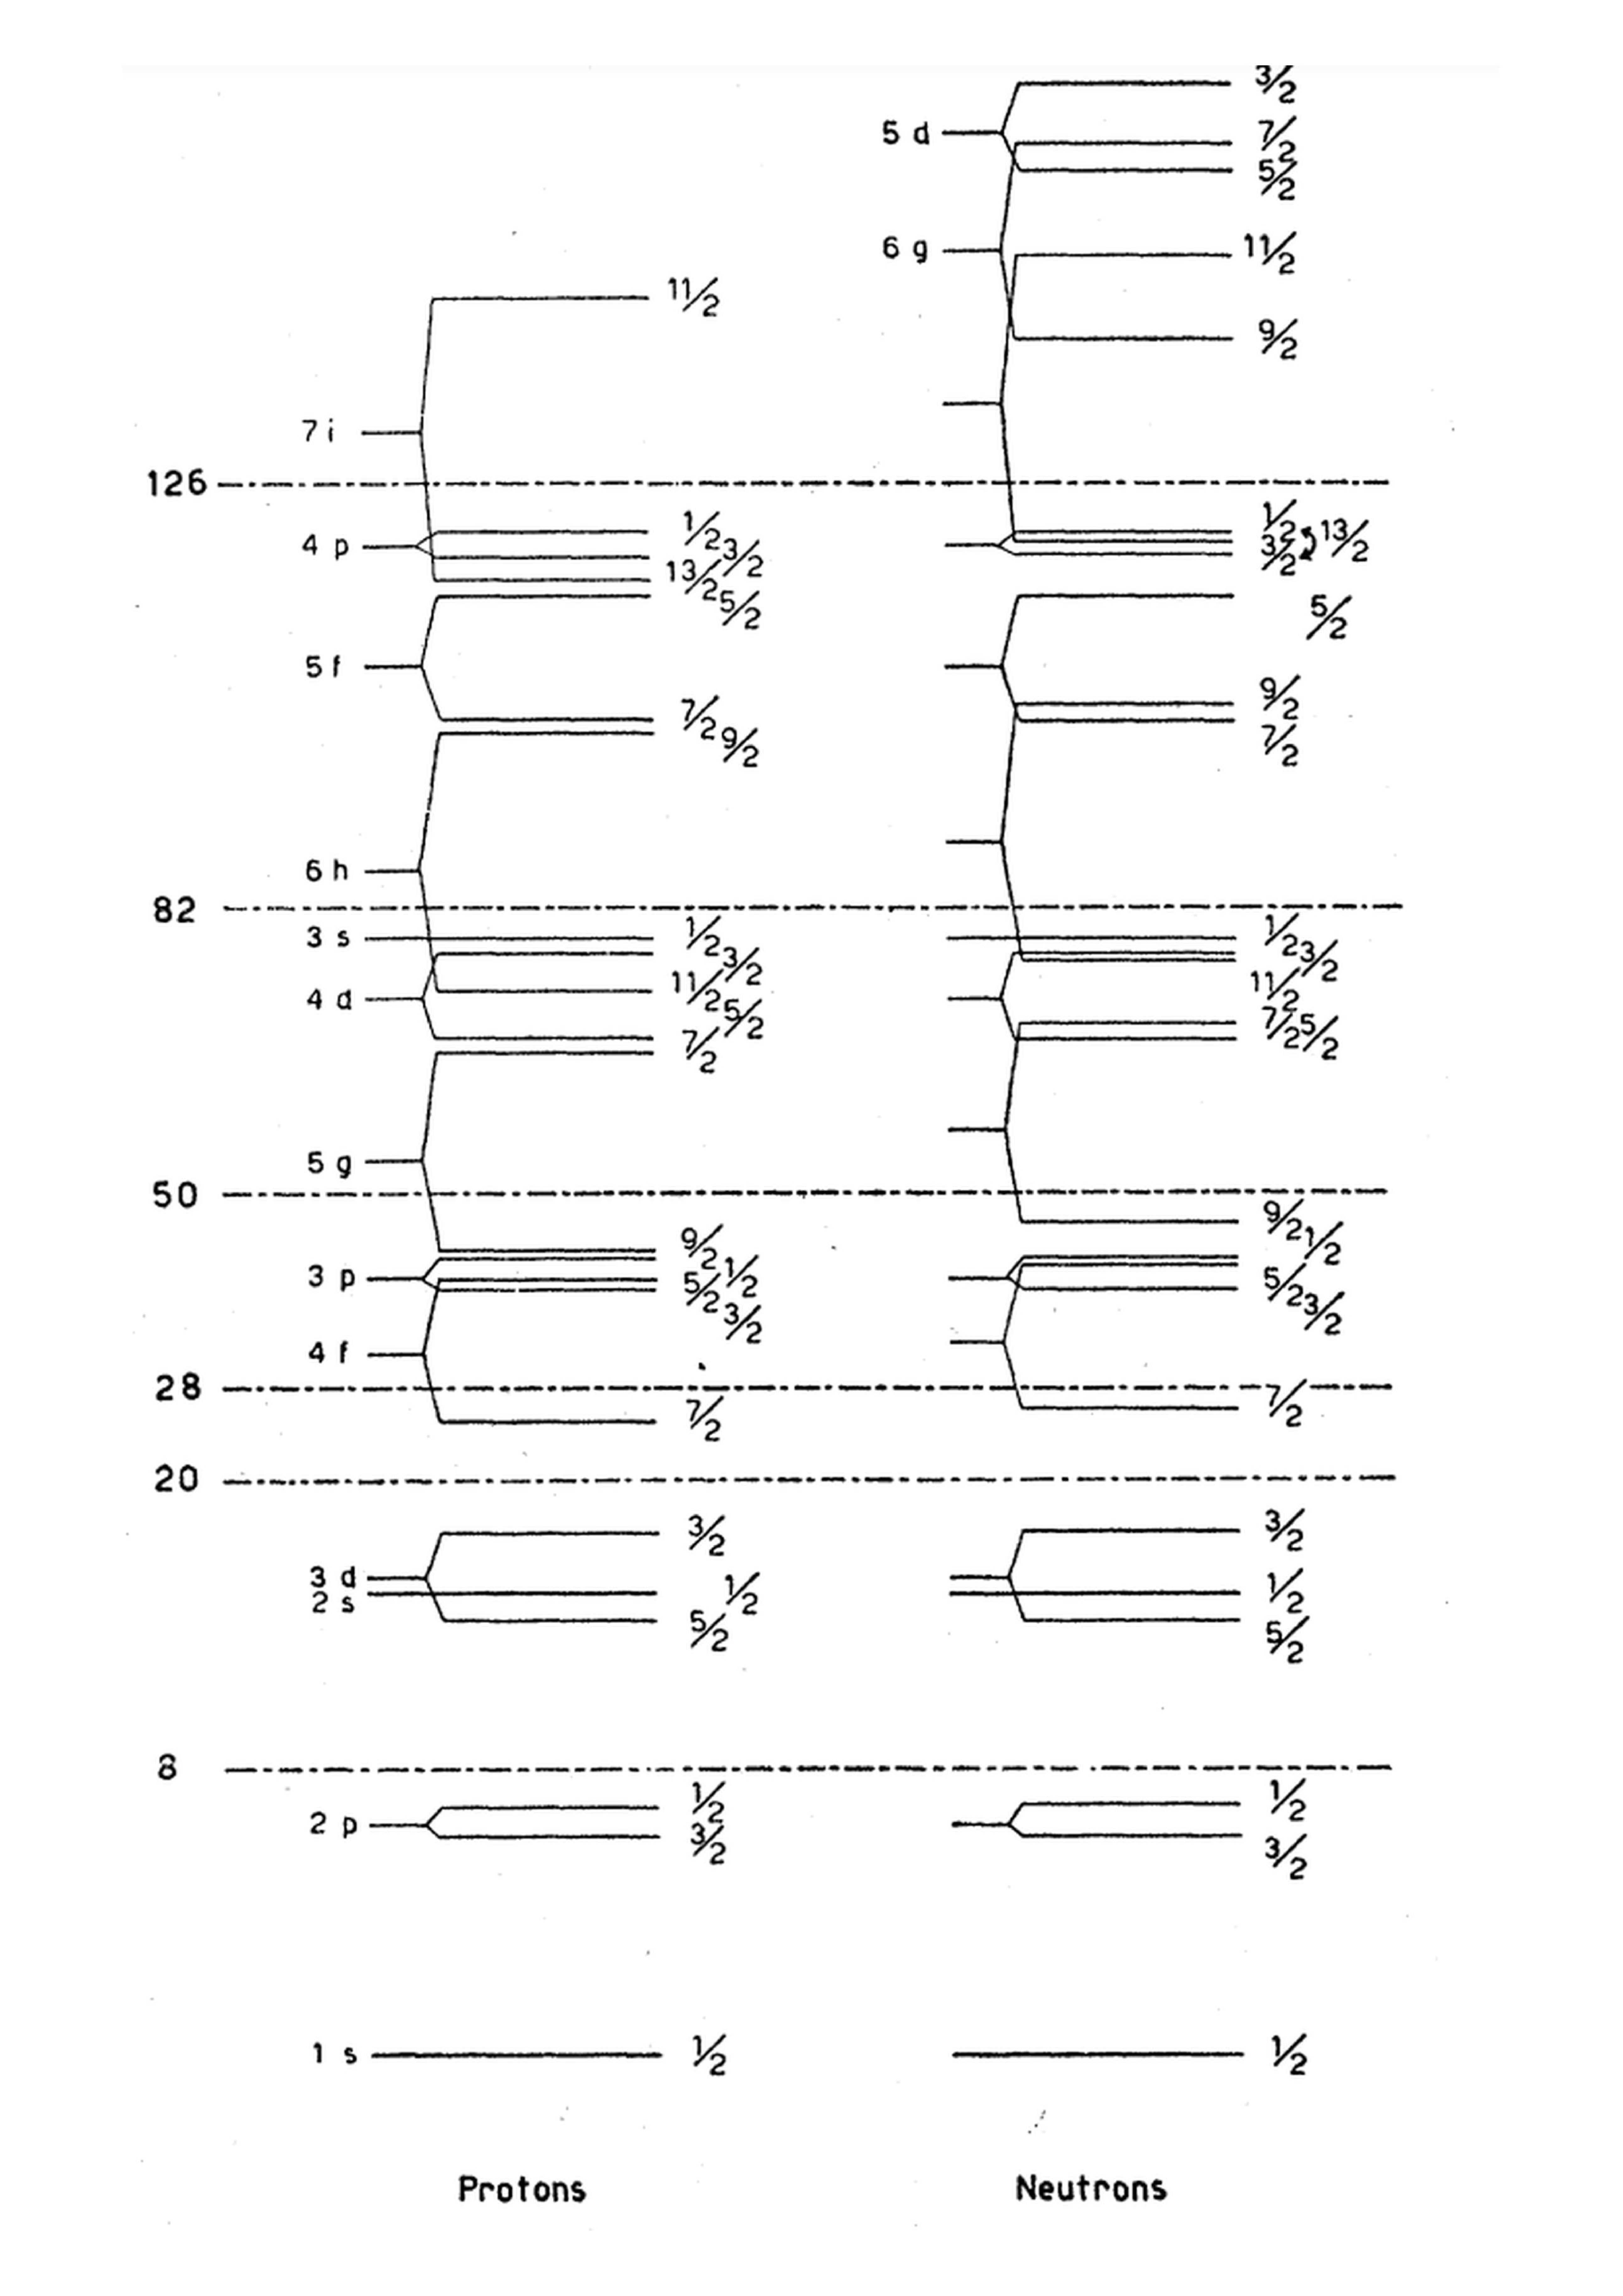
\includepdf[pages=1]{Diagramas Tema 5/Niveles energia modelo de capas.pdf}

\section{Predicciones del modelo de capas. Regla de Nordheim}
Para determinar la $J^P$ de los núcleos a partir del modelo de capas utilizaremos el \textbf{modelo extremo de partícula independiente}. la secuencia de niveles del modelo de capas se va llenando por orden creciente de energía. En el modelo de partícula independiente las propiedades del núcleo vienen determinadas únicamente por el nucleón desapareado, por lo tanto
\begin{equation*}
    J=j \quad \text{donde} \quad P=(-)^l, l=j\pm \frac{1}{2}
\end{equation*}

por lo que el momento angular orbital fija el valor de la paridad del núcleo. \\\\
Este modelo funciona muy bien cerca de la capa cerrada y falla para $A<150$ y $190<A<220$, que en esencia son núcleos muy poco esféricamente simétricos.\\\\
Lejos de capa cerrada el nucleón desapareado también determina las propiedades del núcleo, pero las fuerzas residuales no incluidas en el potencial central efectivo producen fuerzas de emparejamiento muy intensas que modifican los niveles energéticos y acoplan nucleones por pares a $J^P=0^+$
\begin{tcolorbox}[colback=airforceblue!20, colframe=airforceblue, title={Ejemplo: $J^P$ de los isótopos $^{15}\mathrm{O}$ y $^{17}\mathrm{O}$}]
    Experimentalmente medimos que $J^P\qty(^{15}_8\mathrm{O}_7)=\nicefrac{1}{2}^-$ y $J^P\qty(^{17}_8\mathrm{O}_9)=\nicefrac{5}{2}^+$, utilizando el modelo de capas tenemos 
    $$\begin{aligned}
        &^{15}_8\mathrm{O}_7 \xrightarrow[]{} 1p_{\nicefrac{1}{2}} \left \{ \begin{aligned}
            &l=1 \Rightarrow P=-\\
            &j=\nicefrac{1}{2}
        \end{aligned} \right. \Rightarrow J^P=\frac{1}{2}^-\\
        &^{17}_8\mathrm{O}_9 \xrightarrow[]{} 1d_{\nicefrac{5}{2}} \left \{ \begin{aligned}
        &l=2 \Rightarrow P=+ \\
            &j=\nicefrac{5}{2}
        \end{aligned} \right. \Rightarrow J^P=\frac{5}{2}^+
    \end{aligned}$$

    El modelo de capas extremo de partícula independiente es capaz de predecir correctamente la $J^P$ de la mayor parte de los estados fundamentales de los estados con $A$ impar.
\end{tcolorbox}
\subsection{Regla de Nordheim}

EL modelo de capas se  puede utilizar también para obtener información acerca del spin del estado fundamental de núcleos impar-impar. Para eso se utiliza la regla de Nordheim. Llamemos $j_p$ y $l_p$ al spin y al momento angular orbital del protón desapareado y $j_n$ y $j_n$ a los del neutrón desapareado. Así, definimos al número de Nordheim como
\begin{equation}
    N_\mathrm{Nord}=j_p-l_p+j_n-l_n
    \label{eq: numero de nordheim}
\end{equation}

La paridad del núcleo vendrá dada por $P=(-)^{l_n}(-)^{l_p}$. La regla de Nordheim dice 
\begin{itemize}
    \item Si $N_\mathrm{Nord}=0 \Rightarrow J=\abs{j_n-j_p}$, por lo que el spin del protón y del neutrón están antiparalelos y por tanto el núcleo va a intentar poner arriba el neutrón.
    \item Si $N_\mathrm{Nord}=\pm 1 \Rightarrow J=\abs{j_n-j_p}$ ó $j_n+j_p$ en este caso los spines ya son paralelos.
\end{itemize}

La regla de Nordheim, aplicable a núcleos con más de un nucleón fuera de capas cerradas, fue confirmada de forma teórica por De Shalit y Walecka.

\section{Momento dipolar magnético. Líneas de Schmidt}
El modelo de partícula independiente predice que el momento dipolar magnético de un núcleo con $A$ impar es debido exclusivamente al nucleón desapareado. El momento dipolar magnético en unidades del magnetón nuclear es (ecuación \ref{eq: momento magnetico})
\begin{equation}
    \frac{\vec{\mu}}{\mu_N}=\sum_{i=1}^A \qty(g_i^{(l)}\vec{l}_i+g_i^{(s)}\vec{s}_i) \Rightarrow \frac{\vec{\mu}}{\mu_N}=g_j^{(l)}\vec{l}_j+g_j^{(s)}\vec{s}_j
    \label{eq: momento dipolar nucleon desapareado}
\end{equation}

Por definición, sabemos que el valor esperado del momento magnético en el estado de máxima proyección es 
$$\begin{aligned}
    &\mel{jj}{\vec{\mu}}{jj}=\mel{jj}{g^{(l)}\vec{l}+g^{(s)}\vec{s}}{jj}=\mel{jj}{g^{(l)}l\textcolor{red}{+g^{(l)}s-g^{(l)}s}+g^{(s)}s}{jj}=\\&g^{(l)}\mel{jj}{j}{jj}+ \qty(g^{(s)}-g^{(l)}) \mel{jj}{s}{jj}=g^{(l)}j+\qty(g^{(s)}-g^{(l)})\qty(\pm j\frac{1}{2j+1})
\end{aligned}$$
Por lo que la ecuación \ref{eq: momento dipolar nucleon desapareado} será
\begin{equation}
    \frac{\vec{\mu}}{\mu_N}=\qty(g^{(l)}+\qty(g^{(s)}-g^{(l)})\qty(\pm \frac{1}{2l+1}))j
    \label{eq: resultado momento dipolar magnetico nucleon desapareado}
\end{equation}

Donde hemos utilizado el Teorema de Proyección\footnote{Tenemos que $$\expval{s}=\frac{\expval{\vec{s}\cdot \vec{j}}}{\expval{j^2}}\expval{j}, \quad \expval{\vec{s}\cdot \vec{j}}=\frac{1}{2}\qty(\expval{j^2}-\expval{s^2}-\expval{l^2})=\frac{\hbar^2}{2}\qty(j(j+1)+\frac{3}{4}-l(l+1))$$ como $j=l\pm \nicefrac{1}{2}$, $$\expval{s}=\left \{ \begin{aligned}
    &j=l+\frac{1}{2}\Rightarrow \frac{j}{2l+1}\\
    &j=l-\frac{1}{2}\Rightarrow -\frac{j}{2l+1}
\end{aligned} \right.$$} para obtener este resultado.\\\\
Vamos a recordar que las razones giromagéticas de los nucleones son $$
g_i^{(l)}= \left \{\begin{aligned}
    &g_p^{(l)}=1 \\
        &g_n^{(l)}=0
    \end{aligned} \right. \quad \quad \quad g_i^{(s)}= \left \{\begin{aligned}
        &g_p^{(s)}=5.58 \\
        &g_n^{(s)}=-3.82 \end{aligned} \right.$$
\newpage
\noindent

\subsection{Líneas de Schmidt}
En las siguientes figuras hemos representado los valores calculados como líneas sólidas, conocidas como \textbf{líneas de Schmidt}; realizado por él mismo en 1937.  Los valores experimentales caen con los límites de las líneas de Schmidt, pero normalmente tienen valores menores y presentan más dispersión.
\\\\ Una posible mejora se produce por asumir que el valor de las razones giromagnéticas de los nucleones libres y de los nucleones en el núcleo no tienen porqué ser iguales. Para núcleos ligeros el acuerdo entre modelo y experimento es bastante satisfactorio.

\begin{figure}[h!]
    \centering
    % Subfigura para protones impares
    \begin{subfigure}[b]{0.45\textwidth}
        \centering
        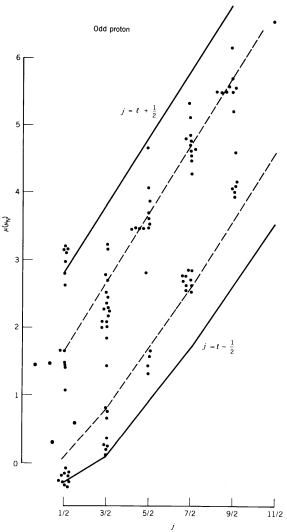
\includegraphics[width=\textwidth]{Diagramas Tema 5/Lineas de Schmidt protones impares.png}
        \caption{Líneas de Schmidt para protones impares.}
        \label{fig:lineas-schmidt-protones}
    \end{subfigure}
    \hfill
    % Subfigura para neutrones impares
    \begin{subfigure}[b]{0.45\textwidth}
        \centering
        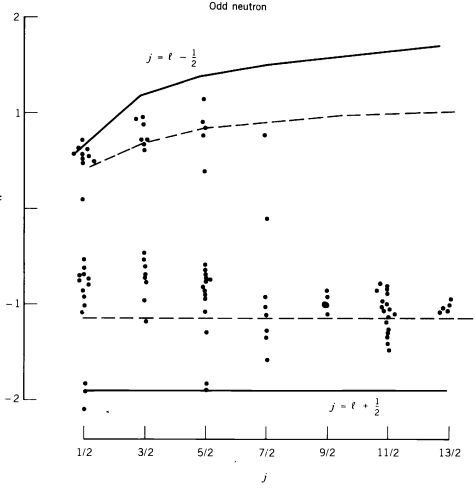
\includegraphics[width=\textwidth]{Diagramas Tema 5/Lineas de Schmidt neutrones impares.png}
        \caption{Líneas de Schmidt para neutrones impares.}
        \label{fig:lineas-schmidt-neutrones}
    \end{subfigure}
    \caption{Líneas de Schmidt para nucleones impares.}
    \label{fig:lineas-schmidt-nucleones}
\end{figure}
